%\begin{frame}
%    \frametitle{Parallel programming}
%    Why parallel processing?
%    \begin{itemize}
%	\item	To get more processing power
%	\item	To get more available memory
%	\item	Future $\rightarrow$ \emph{more} processors rather than faster
%    \end{itemize}
%    \ \\
%    \ \\
%    \ \\
%    \pause
%    Parallelization means
%    \begin{itemize}
%	\item	\textbf{distributing work} among available processors
%	\item	\textbf{syncronizing} distributed work
%	\item	\textbf{distributing data} among available memory
%	\item	\textbf{communicating} distributed data
%    \end{itemize}
%\end{frame}

%\begin{frame}
%    \frametitle{Shared memory (OpenMP)}
%    \begin{columns}
%    \begin{column}[b]{0.45\linewidth}
%	Pros
%	\begin{itemize}
%	    \item Relatively simple implementation
%	    \item Quick way to good performance
%	    \item No communication
%	    \item Simple load balance
%	\end{itemize}
%	\ \\
%	\ \\
%	\pause
%	Cons
%        \begin{itemize}
%	    \item Small to medium scale parallelization
%	    \item Limited memory
%	    \item Race conditions
%	    \item Tedious debugging (Heisenbugs)
%	\end{itemize}
%	\ \\
%	\ \\
%    \end{column}
%    \begin{column}[b]{0.4\linewidth}
%	\only<3>{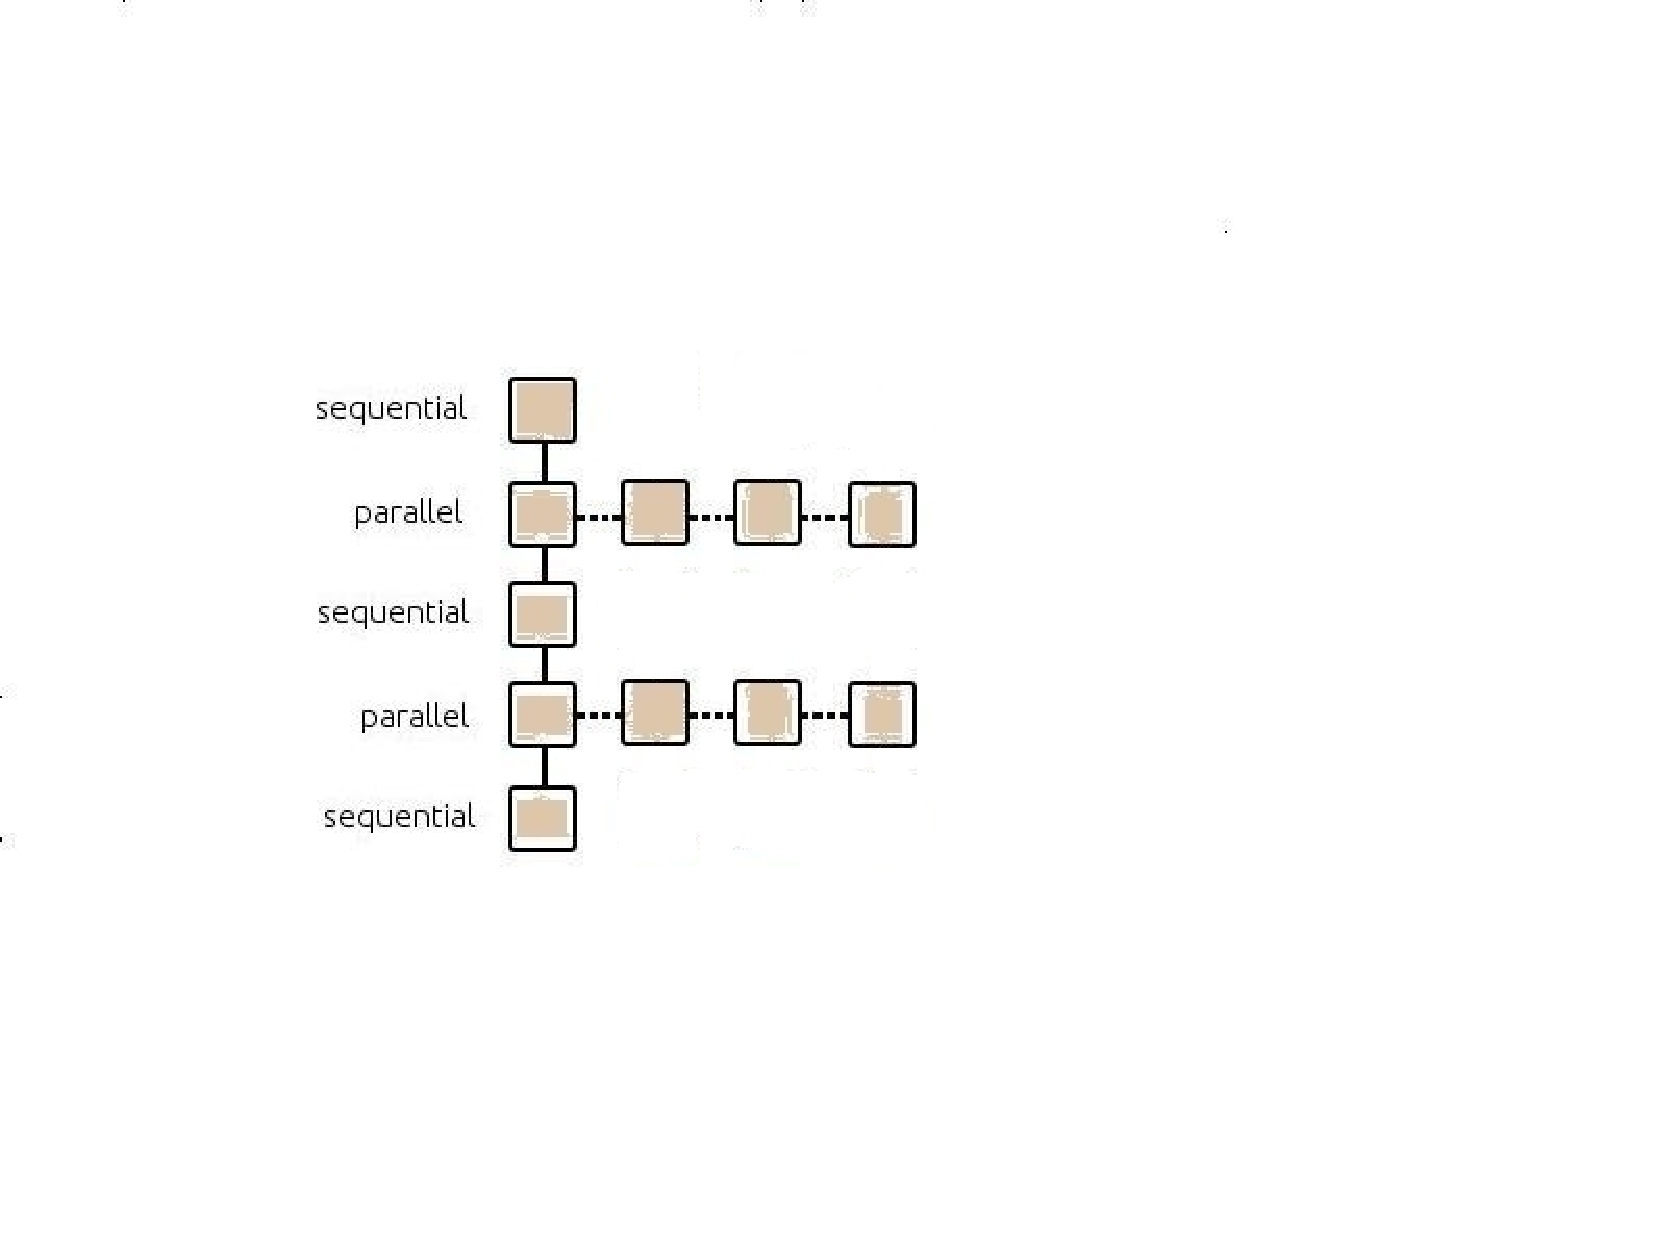
\includegraphics[viewport = 120 160 460 450, clip, scale=0.4]{figures/parallel_OMP.pdf}}
%	\ \\
%	\ \\
%	\ \\
%	\ \\
%    \end{column}
%    \end{columns}
%\end{frame}

%\begin{frame}
%    \frametitle{Distributed memory (MPI)}
%    \begin{columns}
%    \begin{column}[b]{0.45\linewidth}
%	Pros
%	\begin{itemize}
%	    \item Large scale parallelization
%	    \item Extensive memory
%	\end{itemize}
%	\ \\
%	\ \\
%	\ \\
%	\ \\
%	\pause
%	Cons
%	\begin{itemize}
%	    \item Complicated implementation
%	    \item User specified work/data decomposition 
%	    \item User specified communication
%	    \item Difficult to load balance
%	    \item Communication overhead
%	\end{itemize}
%    \end{column}
%    \begin{column}[b]{0.4\linewidth}
%	\only<3>{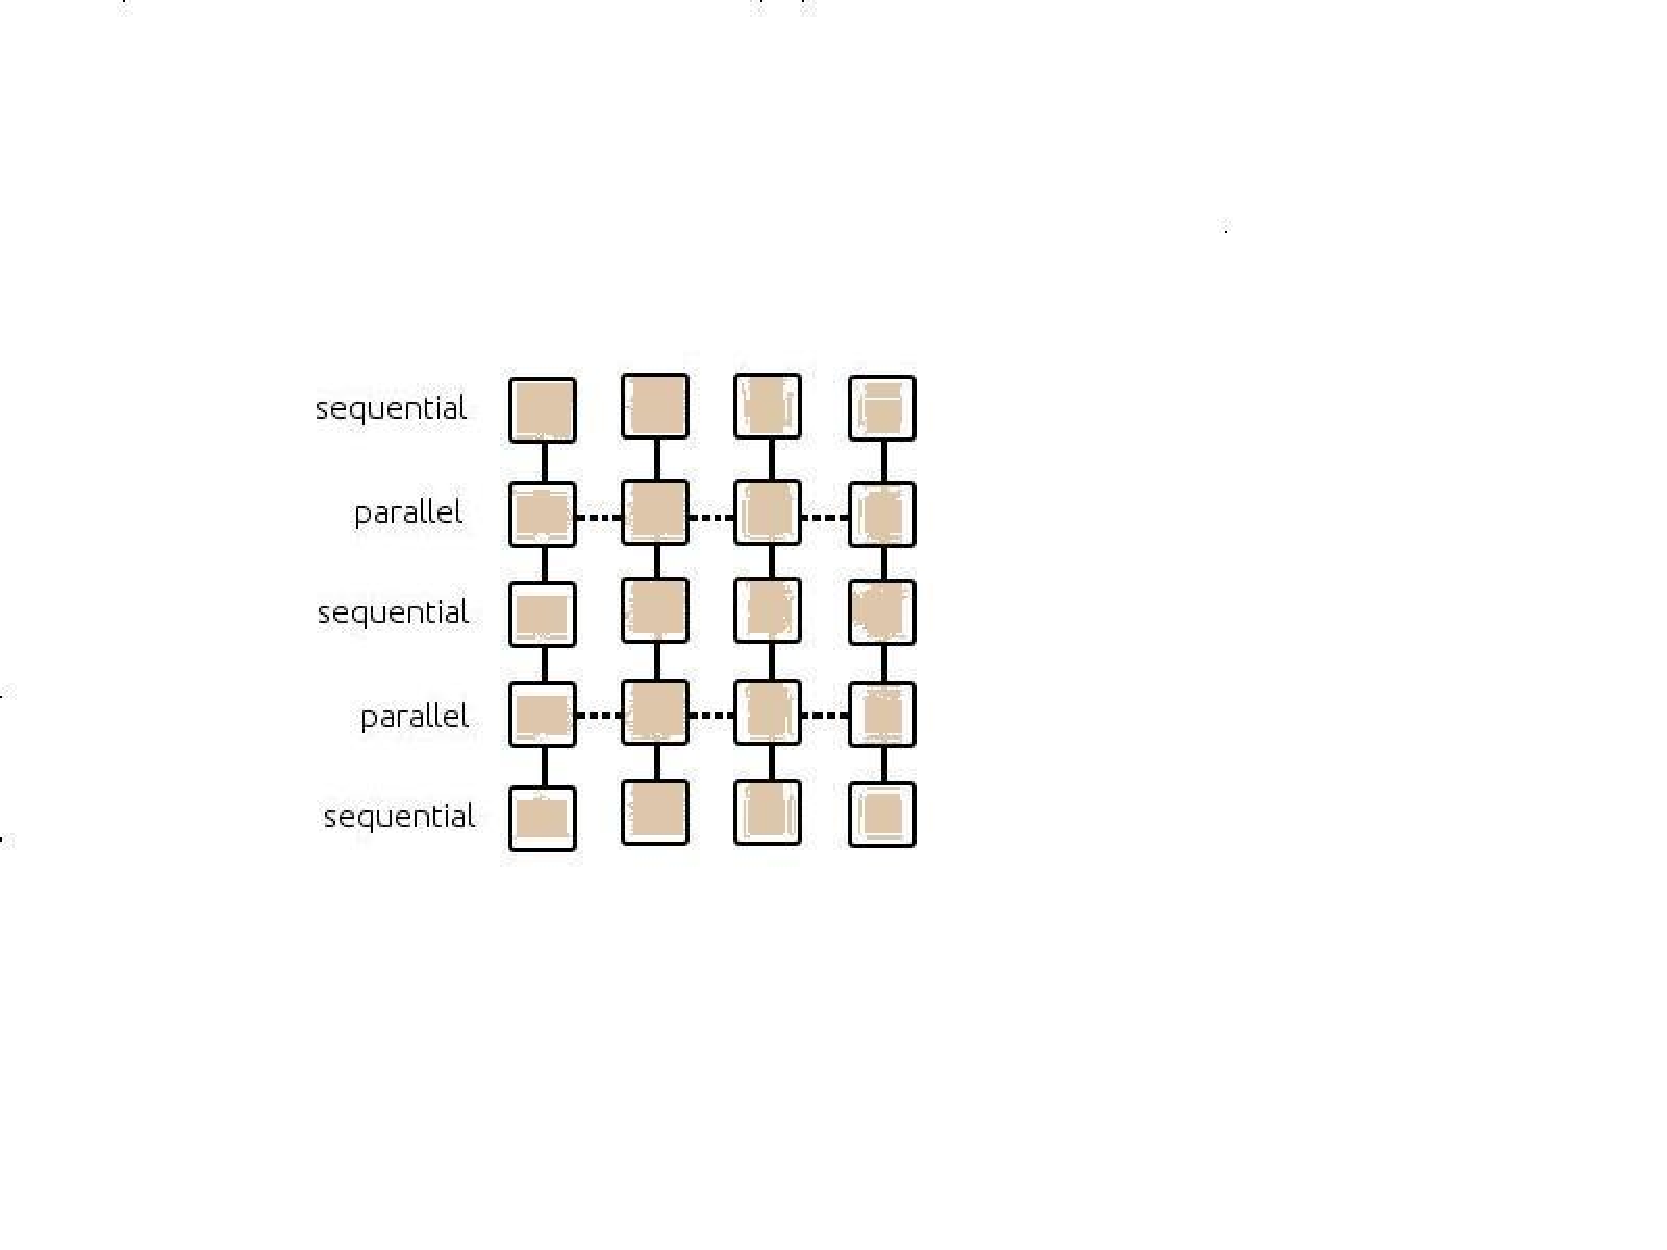
\includegraphics[viewport = 120 160 460 450, clip, scale=0.4]{figures/parallel_mpi_2.pdf}}
%	\ \\
%	\ \\
%	\ \\
%    \end{column}
%    \end{columns}
%\end{frame}
%
%\begin{frame}
%    \frametitle{Parallel efficiency}
%    \begin{center}
%    \only<1>{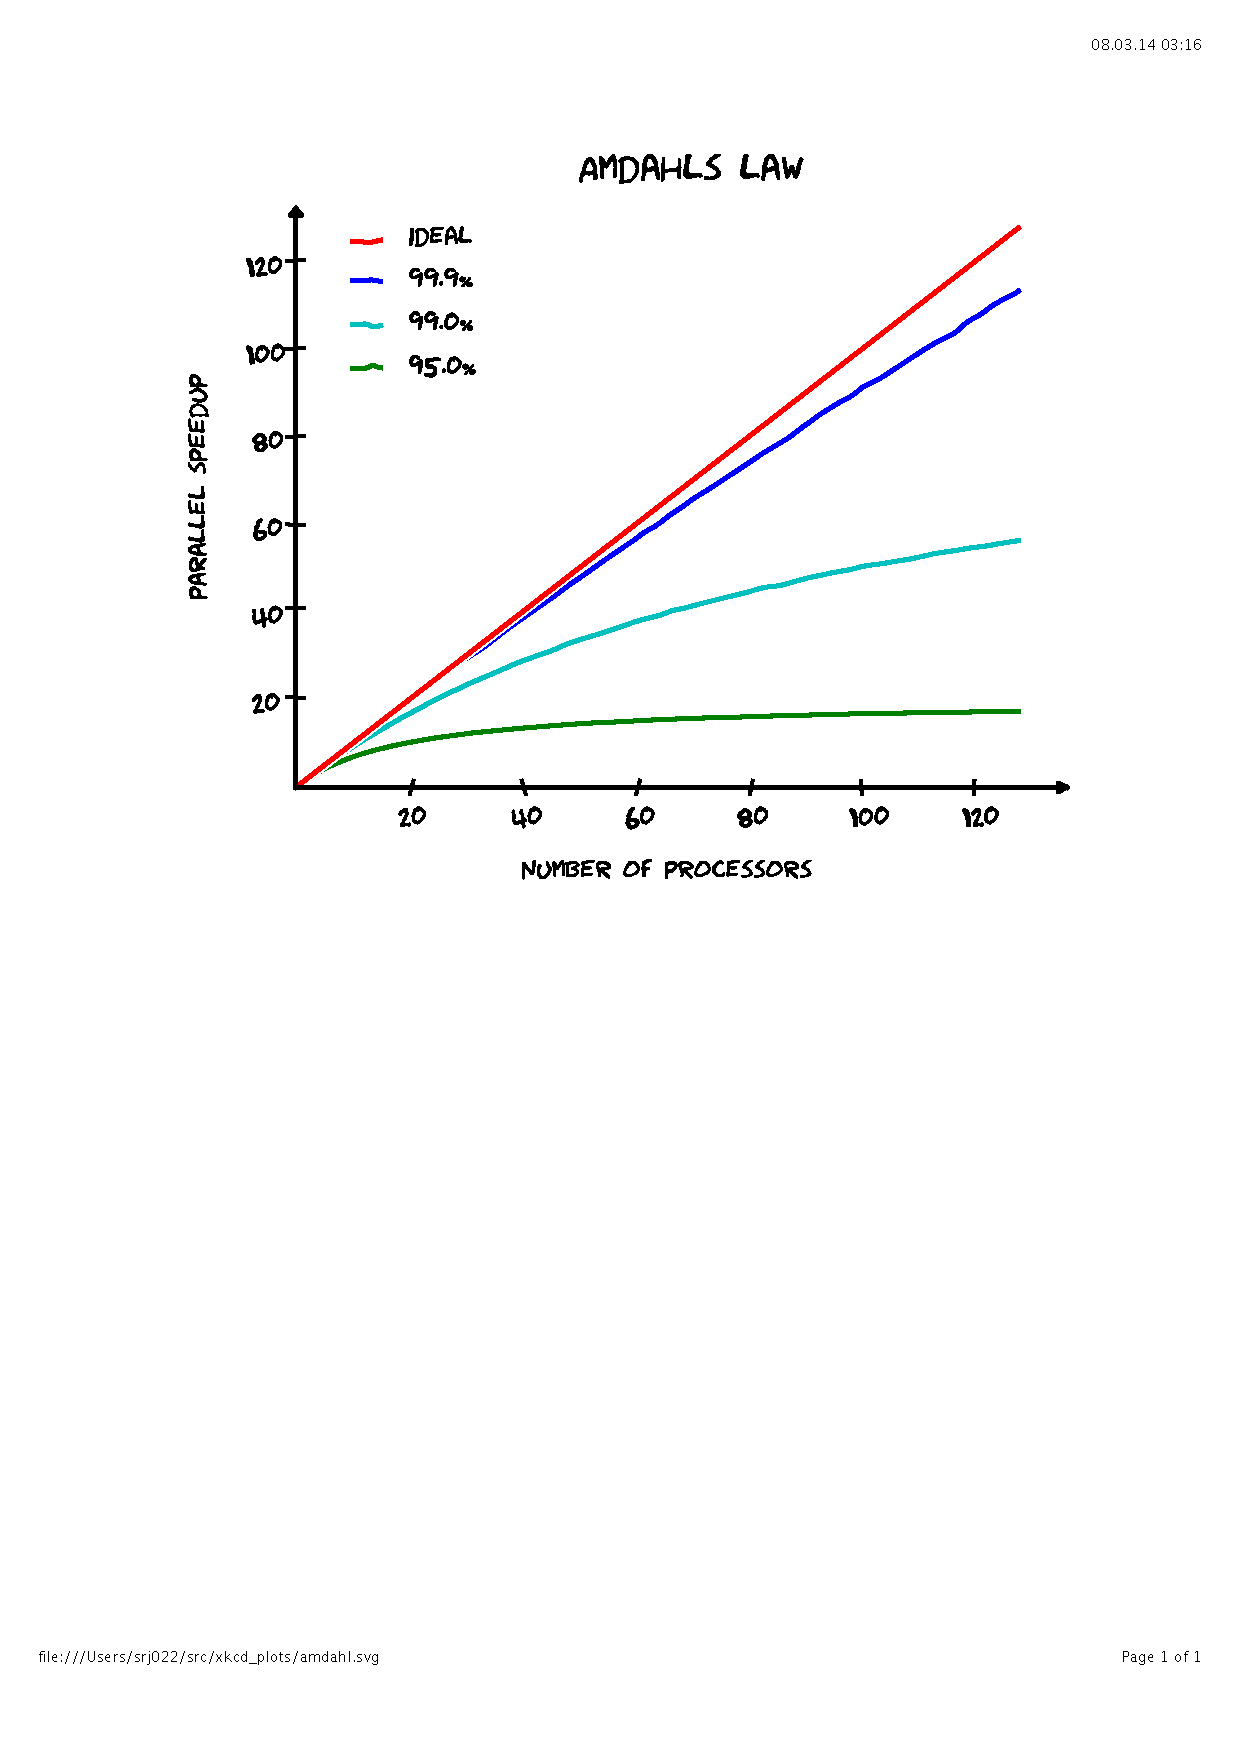
\includegraphics[clip, viewport = 50 250 550 800, scale=0.5]{figures/amdahl.pdf}}
%    \only<2>{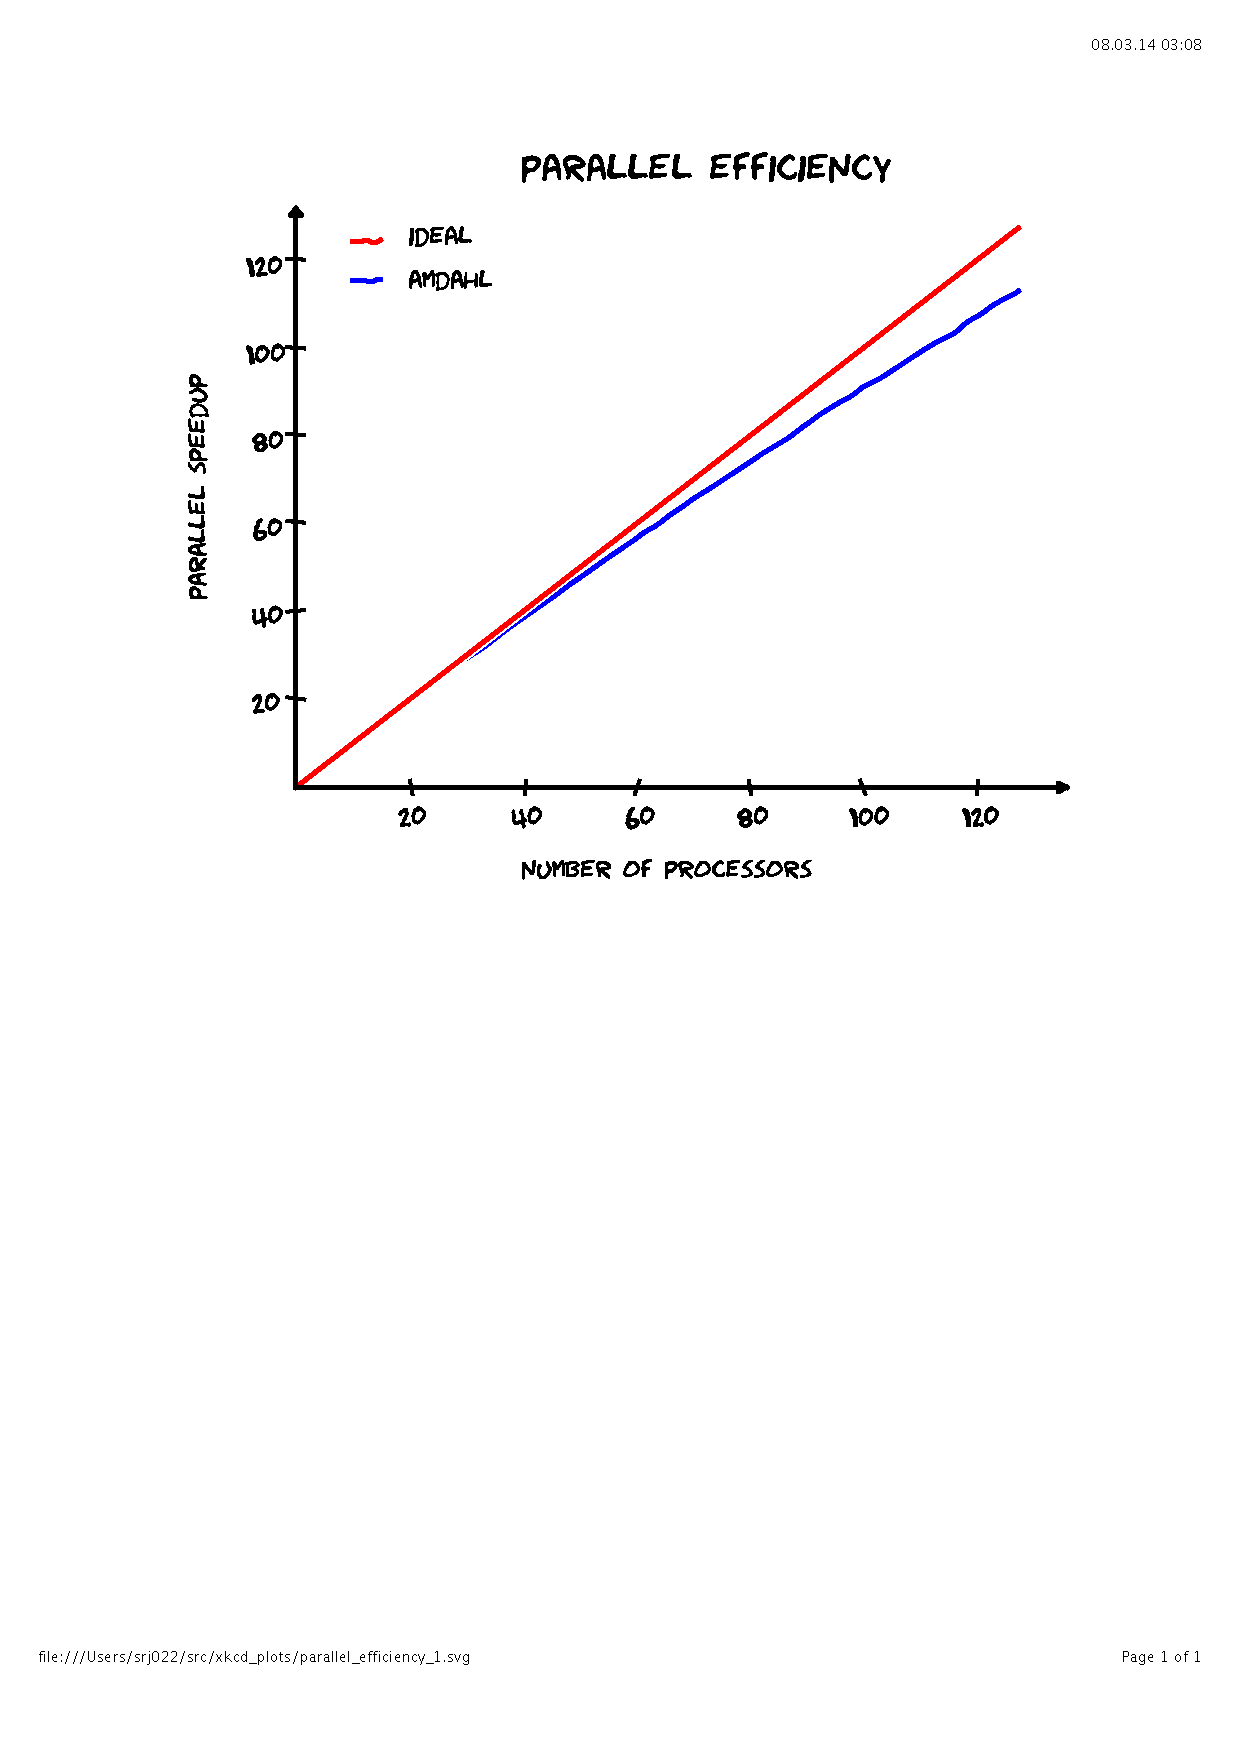
\includegraphics[clip, viewport = 50 250 550 800, scale=0.5]{figures/parallel_efficiency_1.pdf}}
%    \only<3>{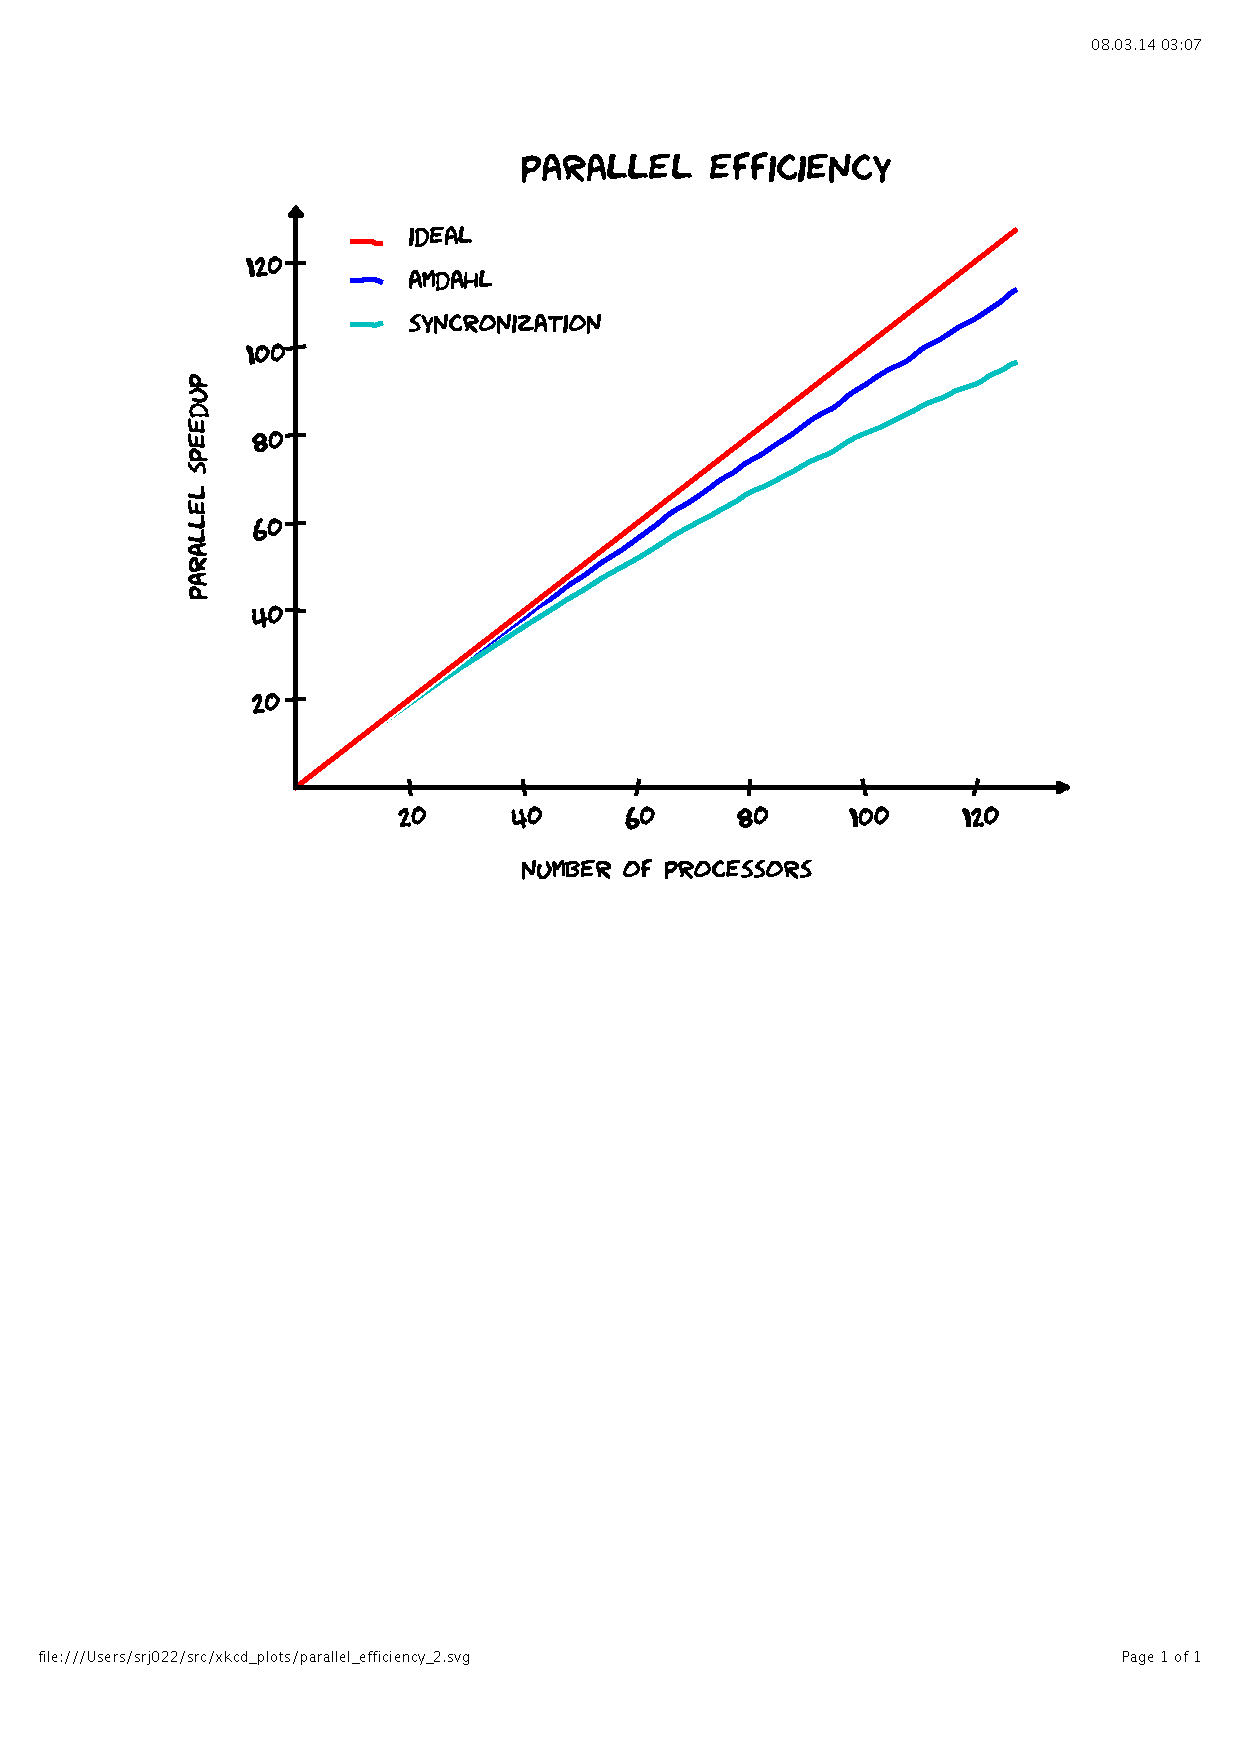
\includegraphics[clip, viewport = 50 250 550 800, scale=0.5]{figures/parallel_efficiency_2.pdf}}
%    \only<4>{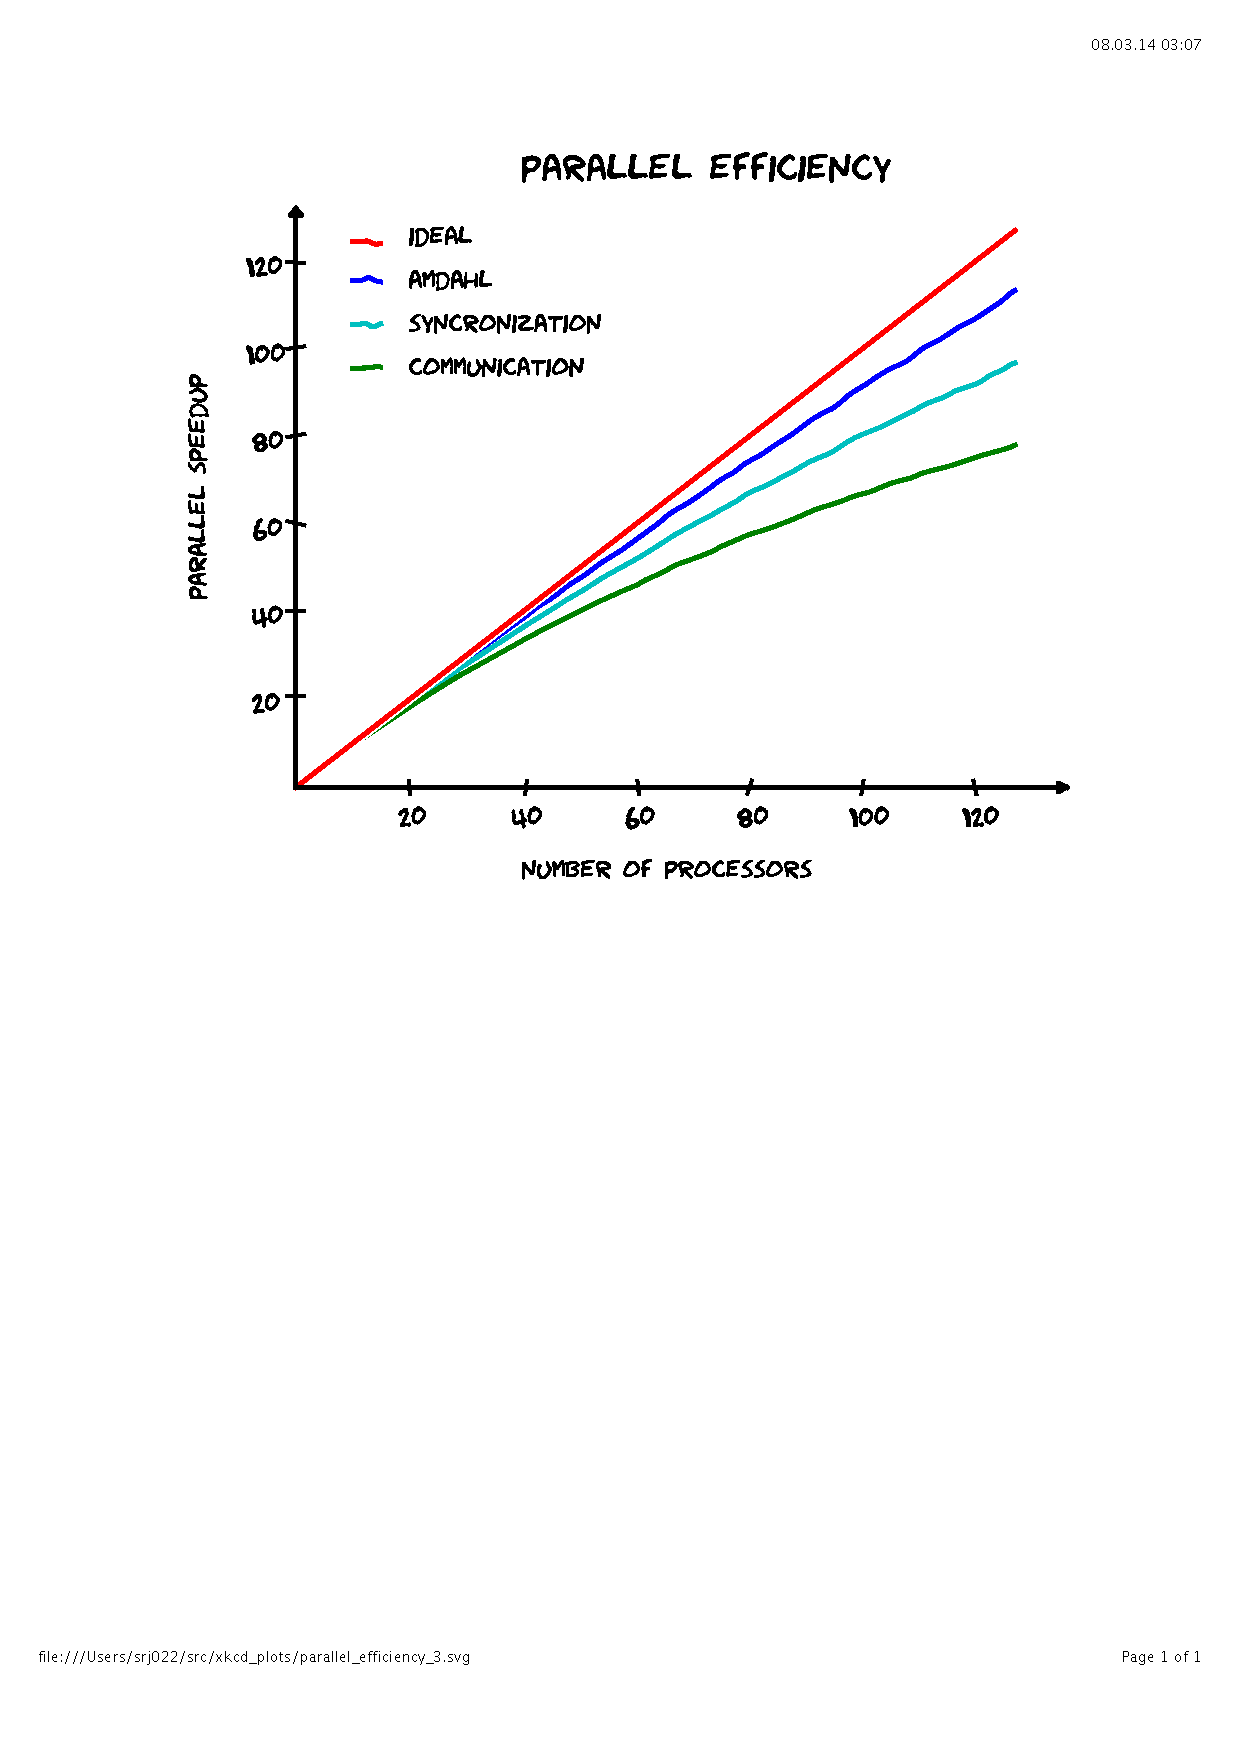
\includegraphics[clip, viewport = 50 250 550 800, scale=0.5]{figures/parallel_efficiency_3.pdf}}
%    \end{center}
%\end{frame}

%\begin{frame}
%    \frametitle{Parallelization}
%    \begin{columns}
%    \begin{column}{.5\textwidth}
%	\ \ \ \ \textbf{Shared memory using OpenMP}
%	\begin{itemize}
%	    \item All CPUs have access to the \textbf{full} grid
%	    \item No communication needed
%	    \item Small scale parallelization ($<50$ CPUs)
%	    \item Work (grid cells) dynamically distributed
%	\end{itemize}
%    \end{column}
%    \begin{column}{.5\textwidth}
%	\ \ \ \ \textbf{Distributed memory using MPI}
%	\begin{itemize}
%	    \item Each CPU has access to a \textbf{local} part of the grid
%	    \item Communication required
%	    \item Large scale parallelization ($>1000$ CPUs)
%	    \item Work (grid cells) distributed \it{a priori}
%	\end{itemize}
%    \end{column}
%    \end{columns}
%    \ \\
%    \ \\
%    \ \\
%    \ \\
%    \begin{columns}
%    \begin{column}{0.4\textwidth}
%	\centering
%	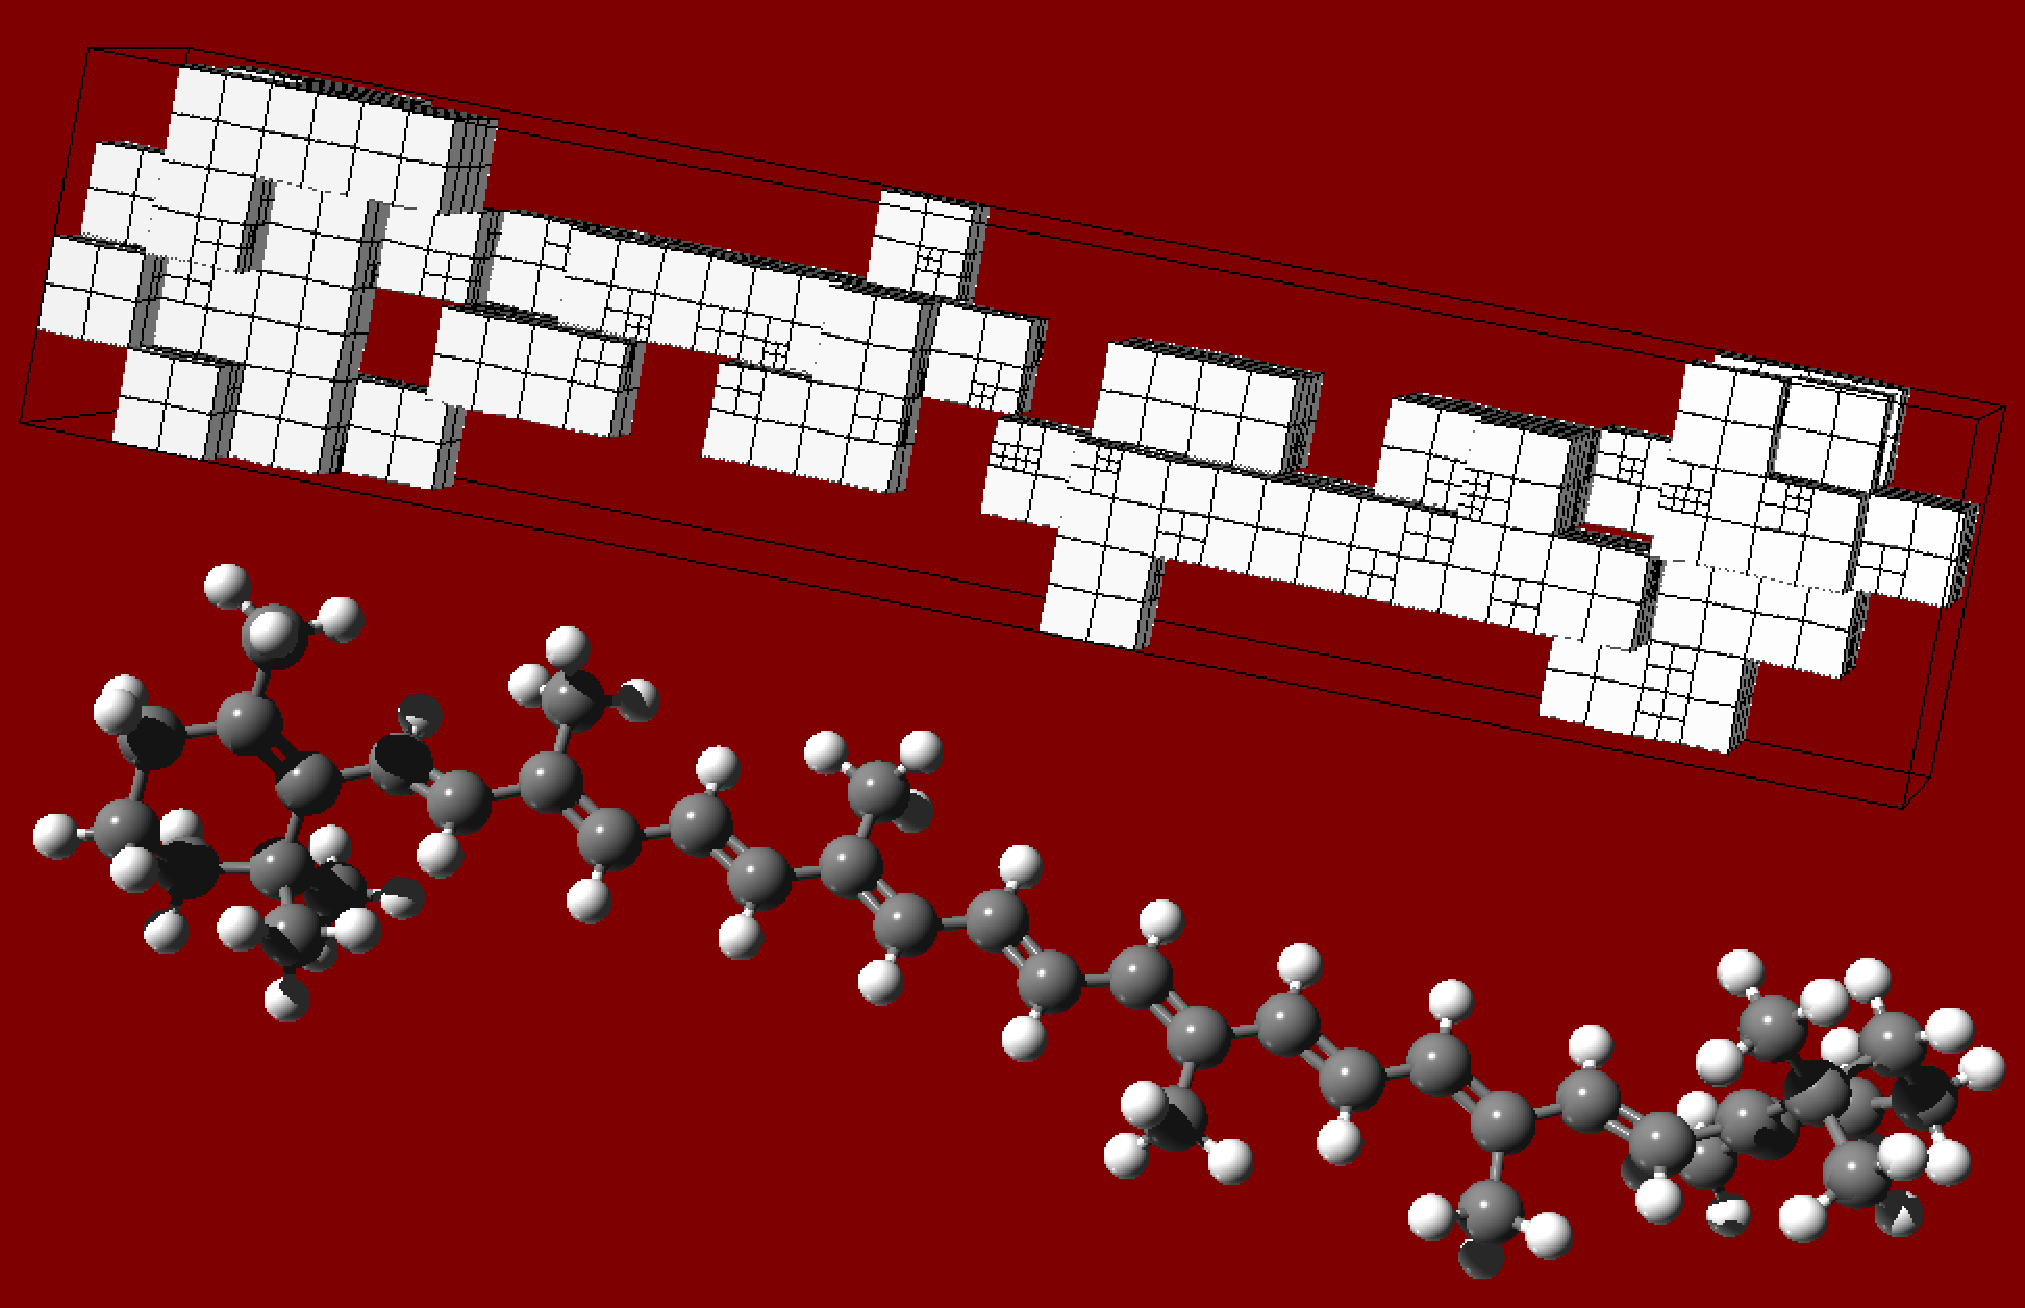
\includegraphics[angle=-90, scale=0.15]{figures/caroteneGrid.pdf}
%    \end{column}
%    \begin{column}{0.6\textwidth}
%	\centering
%	\textbf{Lebesgue path}
%	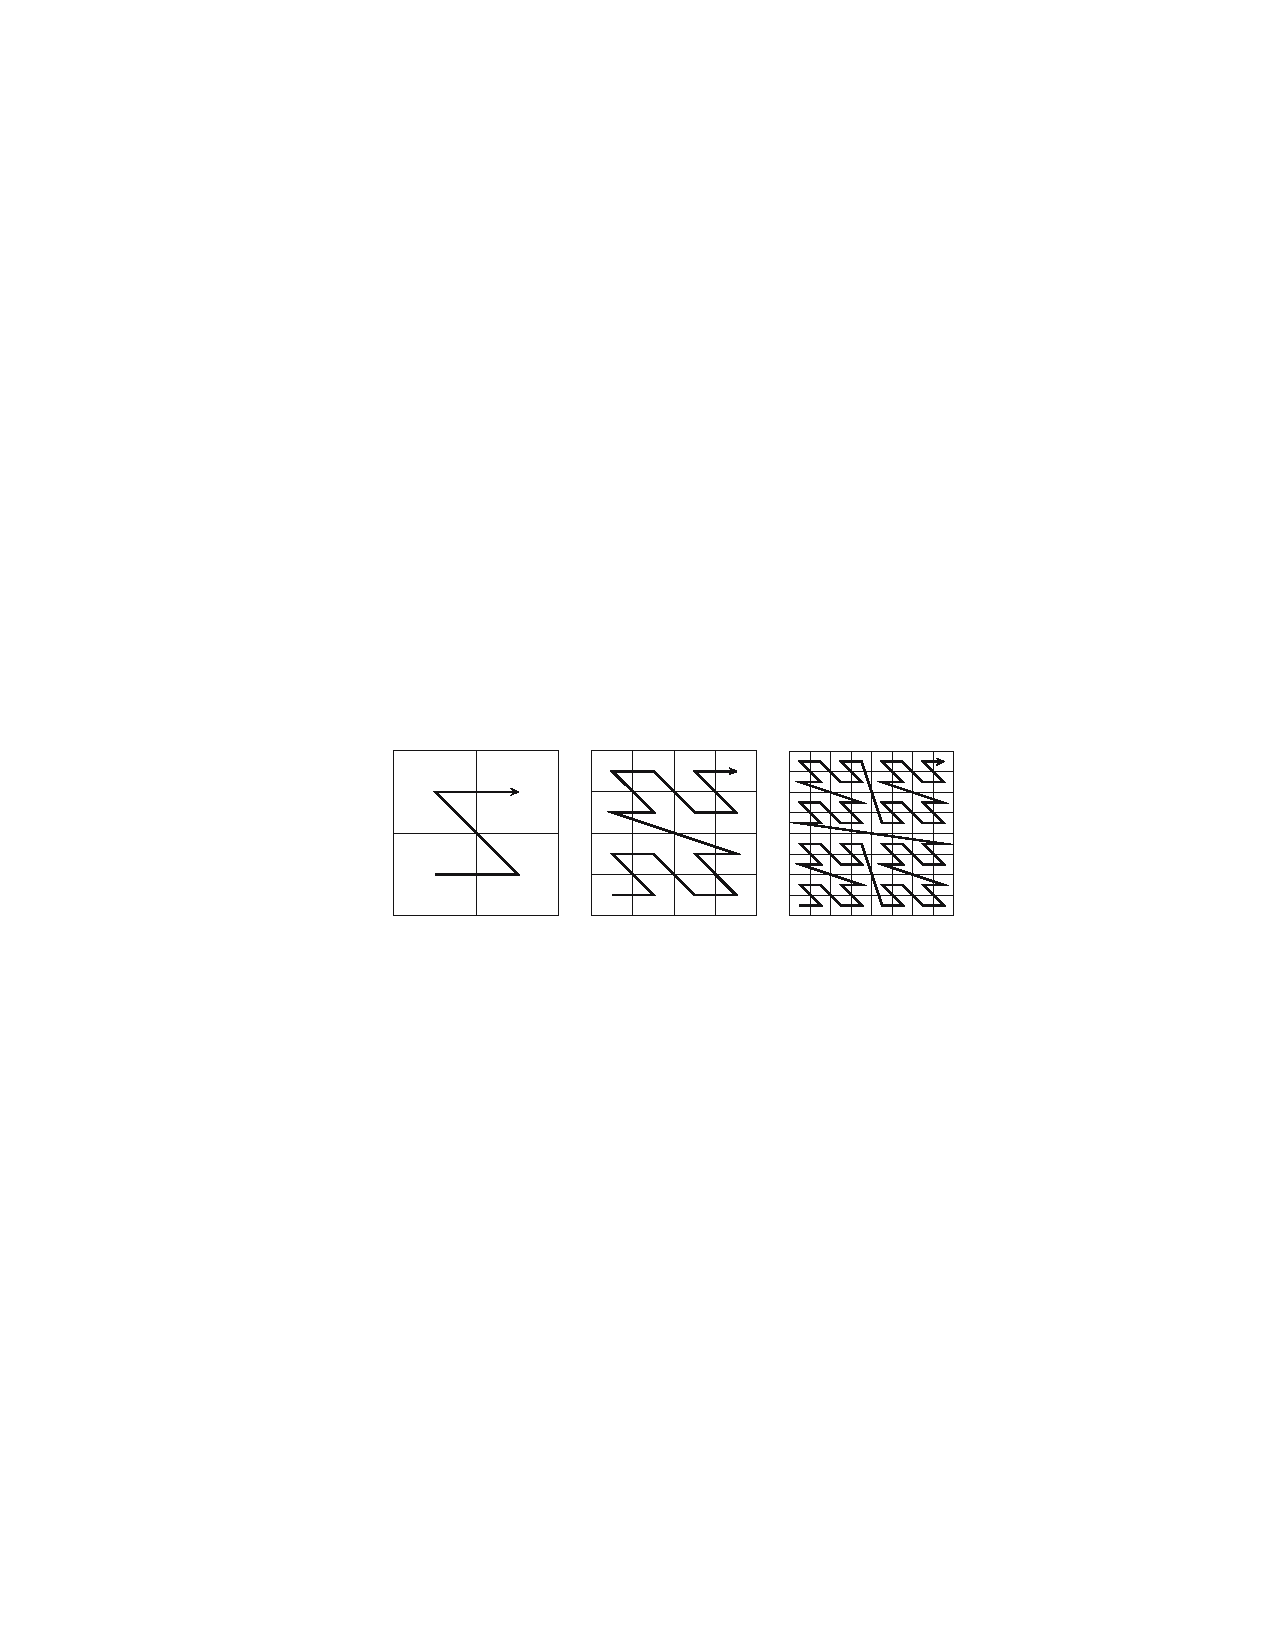
\includegraphics[scale=0.5, viewport = 150 350 500 435, clip]{figures/lebesgue.pdf}
%	\ \\
%	\ \\
%	\ \\
%	\textbf{Hilbert path}
%	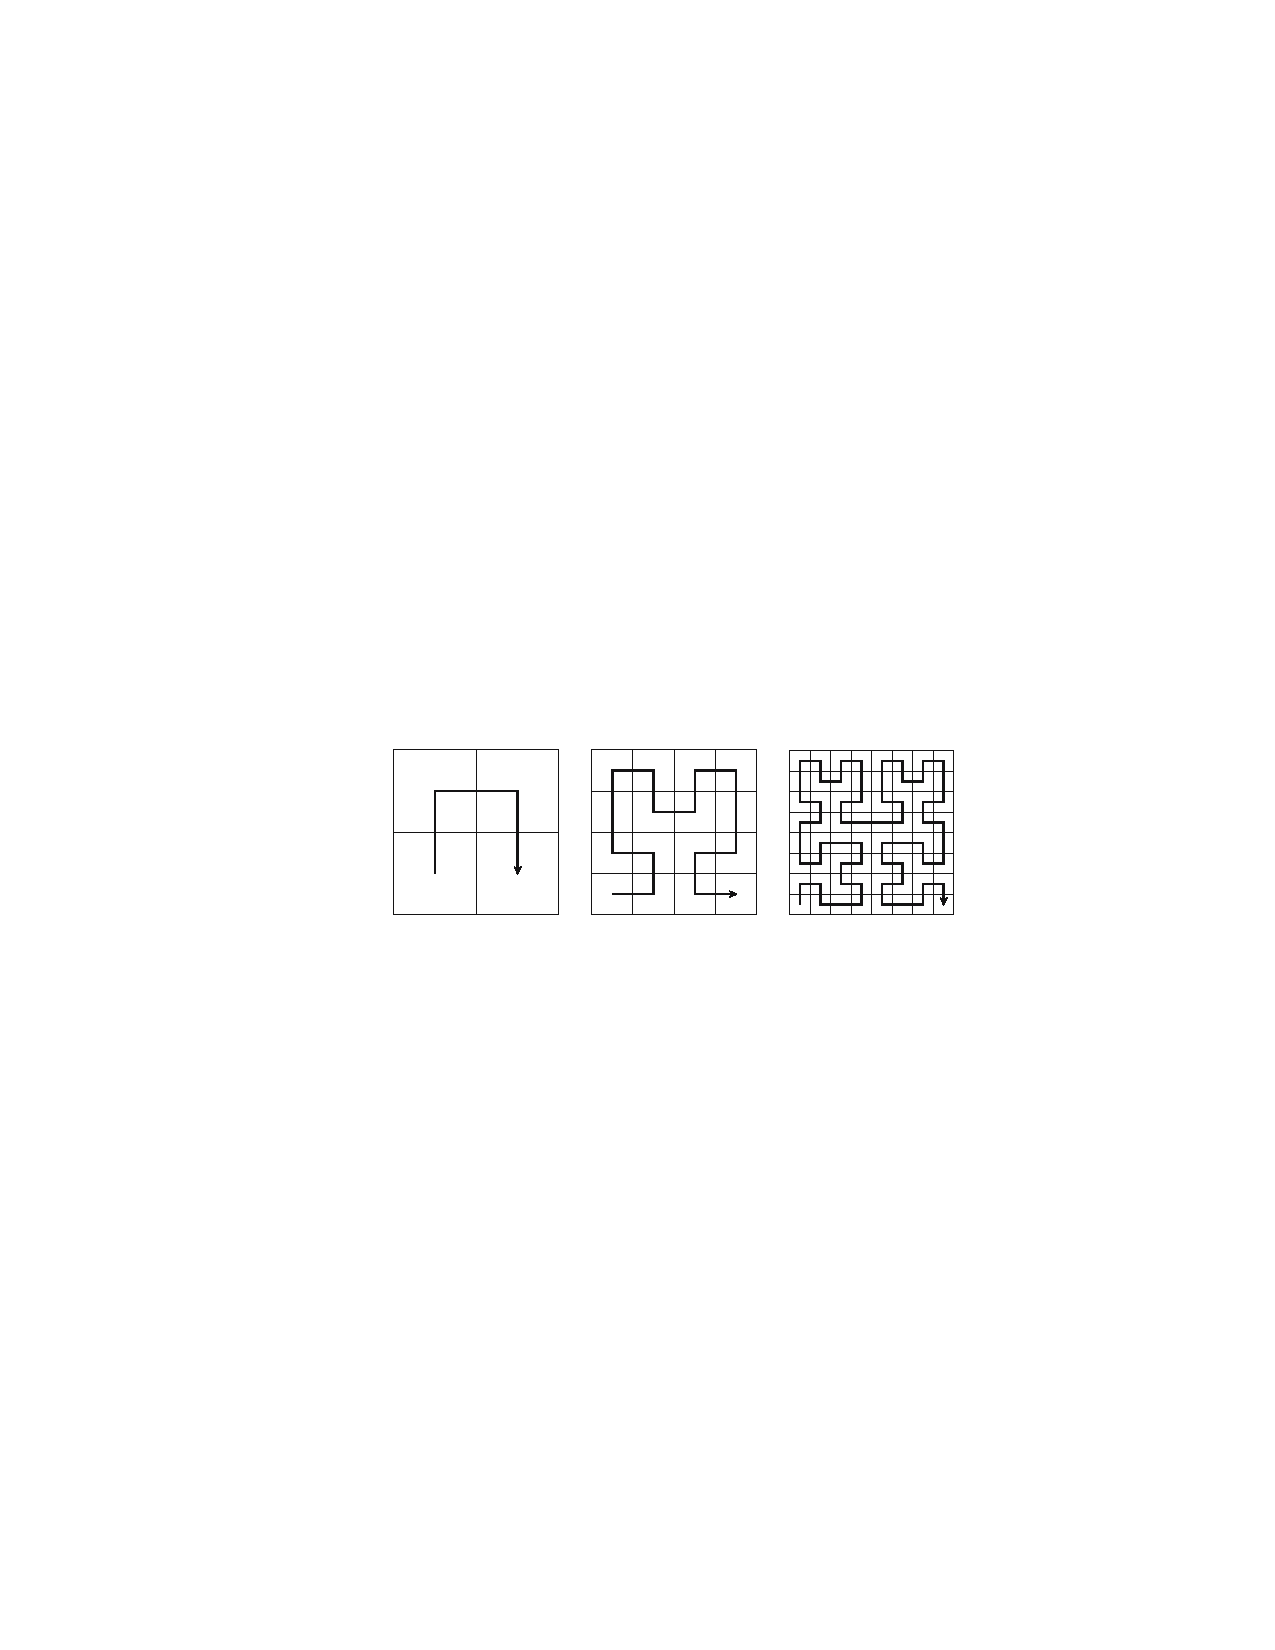
\includegraphics[scale=0.5, viewport = 150 350 500 435, clip]{figures/hilbert.pdf}
%    \end{column}
%    \end{columns}
%\end{frame}

%\begin{frame}
%    \frametitle{Parallelization}
%    \begin{columns}
%    \begin{column}{.5\textwidth}
%	\ \ \ \ \textbf{Shared memory using OpenMP}
%	\begin{itemize}
%	    \item All CPUs have access to the \textbf{full} grid
%	    \item No communication needed
%	    \item Small scale parallelization ($<50$ CPUs)
%	    \item Work (grid cells) dynamically distributed
%	\end{itemize}
%    \end{column}
%    \begin{column}{.5\textwidth}
%	\ \ \ \ \textbf{Distributed memory using MPI}
%	\begin{itemize}
%	    \item Each CPU has access to a \textbf{local} part of the grid
%	    \item Communication required
%	    \item Large scale parallelization ($>1000$ CPUs)
%	    \item Work (grid cells) distributed \it{a priori}
%	\end{itemize}
%    \end{column}
%    \end{columns}
%    \ \\
%    \ \\
%    \ \\
%    \ \\
%    \centering
%    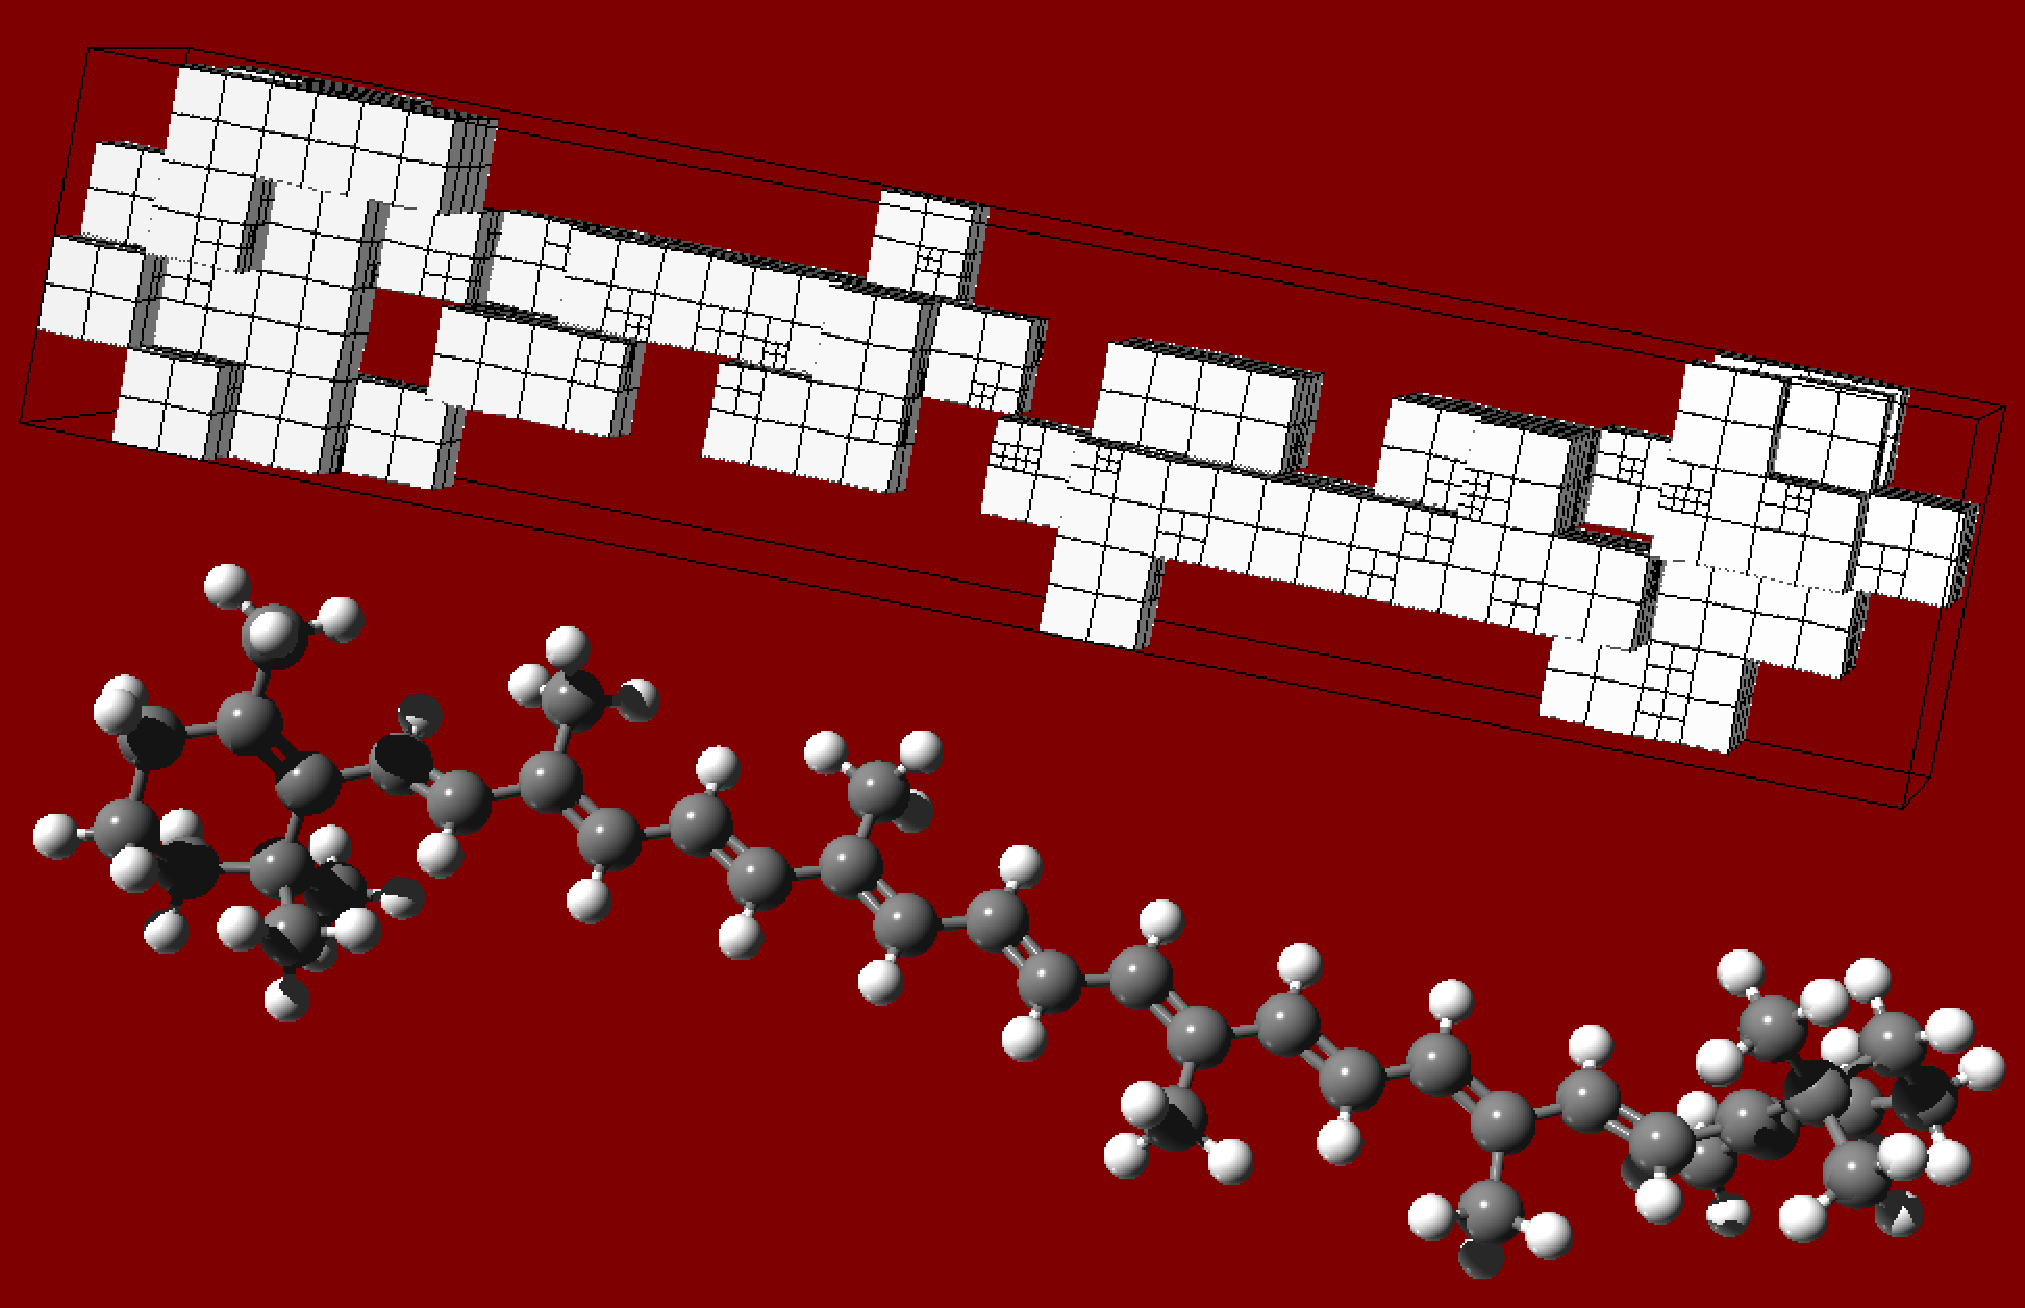
\includegraphics[angle=0, scale=0.2]{figures/caroteneGrid.pdf}
%\end{frame}

\begin{frame}
    \frametitle{Linear scaling and parallel performance}
    \begin{columns}
    \begin{column}{.10\textwidth}
    \ \\
    \end{column}
    \begin{column}{.40\textwidth}
    \centering
    \textbf{Diamond fragments}
    \begin{equation}
	\nonumber
	C_{(2n+3)(n+2)(n+1)/6}H_{2(n+2)(n+1)}
    \end{equation}
    \ \\
    \ \\
    \ \\
    \textbf{Fitted curve}
    \begin{equation}
	\nonumber
	t(n) = 11.6 + 1.84n^{0.805}
    \end{equation}
    \end{column}
    \begin{column}{.50\textwidth}
	\begin{figure}
	    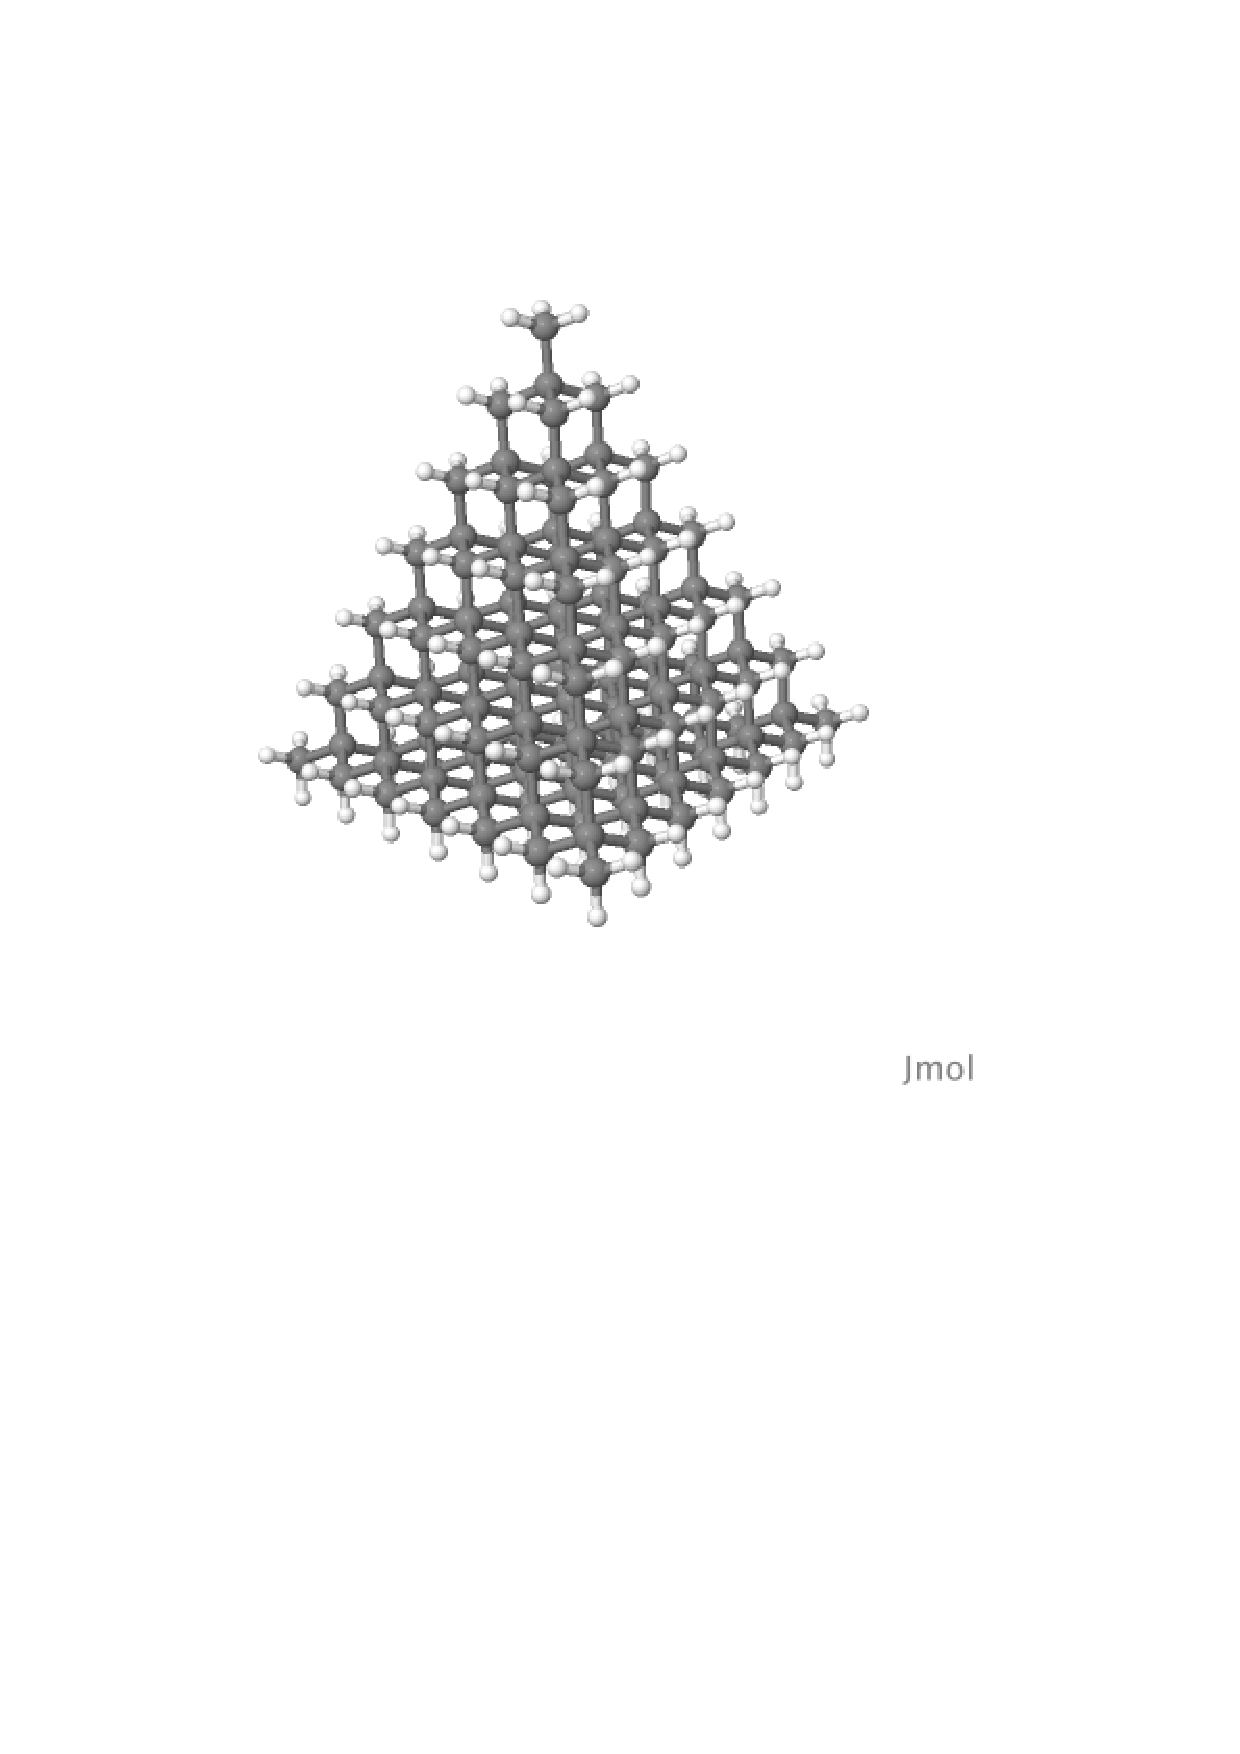
\includegraphics[scale=0.25, clip, viewport = 10 390 500 720]{figures/diamond.pdf}
	\end{figure}
    \end{column}
    \end{columns}    
    \begin{center}
	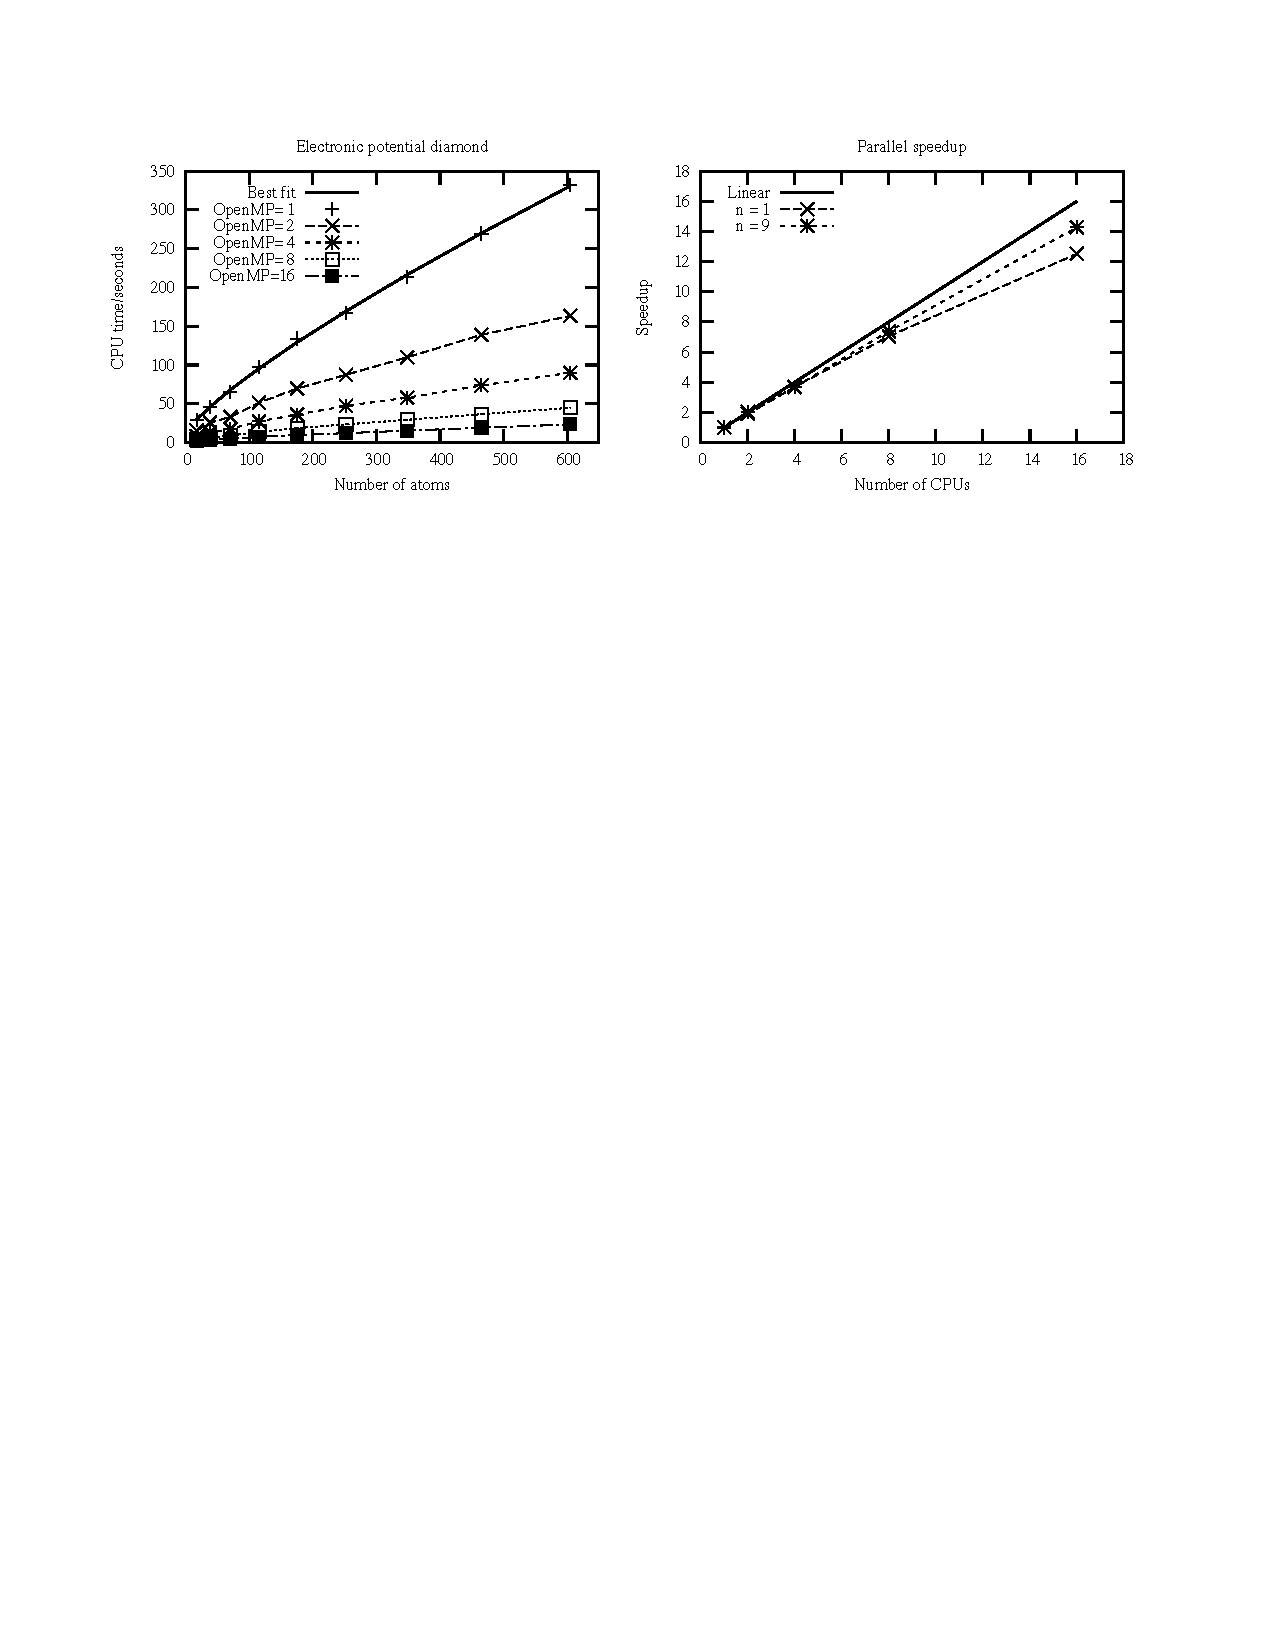
\includegraphics[scale=0.6, clip, viewport = 50 550 540 730]{figures/ompScaling.pdf}
    \end{center}
\end{frame}

\begin{frame}
    \frametitle{Parallel performance}
    \centering
    Wall clock computation time in seconds for parallel calculation of electronic potential\\
    of diamond fragments using pure OpenMP and hybrid MPI/OpenMP strategies.\\
    \begin{table}
    \tiny
    \begin{tabular}{cccrrrrrrrrr}
	\hline
	\hline                                                                           
	\multicolumn{3}{c}{Number of CPUs}&
	\multicolumn{9}{c}{Diamond system $n$ in $C_{(2n+3)(n+2)(n+1)/6}H_{2(n+2)(n+1)}$}\\
	MPI&OMP&TOT	&1	&2	&3	&4	&5	&6	&7	&8	&9	\\
	\hline
	   &   &   	&	&      	&	&	&	&	&	&	&	\\
	  1&  1&  1	& 29.4	& 46.2 	& 64.7 	& 97.8  &133.9  &166.8  &213.4  &269.4  &332.0  \\
	  1&  2&  2	& 15.5	& 25.5 	& 33.0 	& 51.3  & 69.5  & 87.2  &110.0  &138.9  &163.4  \\
	  1&  4&  4	&  8.0 	& 12.8 	& 17.4 	& 27.0  & 36.1  & 47.3  & 57.8  & 73.7  & 90.1  \\
	  1&  8&  8	&  4.2 	&  6.5 	&  8.8 	& 13.9  & 18.6  & 23.5  & 29.4  & 36.7  & 45.0  \\
	  1& 16& 16	&  2.4 	&  3.5 	&  4.7 	&  7.5  &  9.6  & 12.2  & 15.4  & 19.1  & 23.3  \\
%	   &   &   	&      	&      	&    	&    	&    	&	&	&	&	\\
%	  2&  1&  2	& 17.9 	& 28.4 	& 35.8 	& 59.2  & 81.6  & 93.0  &121.7  &147.5  &176.5  \\
%	  4&  1&  4	& 10.1 	& 16.3 	& 21.2 	& 32.5  & 51.6  & 53.8  & 60.8  & 85.3  &100.7  \\
%	  8&  1&  8	&  6.1 	&  9.4 	& 11.8 	& 19.9  & 25.6  & 28.0  & 35.4  & 43.7  & 50.7  \\
%	 16&  1& 16	&  5.0 	&  6.2 	&  8.2 	& 12.4  & 15.0  & 17.3  & 23.0  & 26.1  & 31.3  \\
%	 32&  1& 32	&  3.6 	&  4.2 	&  5.4 	&  9.5  &  9.2  & 10.9  & 14.1  & 16.8  & 20.0  \\
%	 64&  1& 64	&  3.1 	&  3.9 	&  4.3 	&  6.5  &  6.6  &  7.4  & 10.3  & 11.4  & 13.4  \\
%	128&  1&128	&  5.2 	&  5.7 	&  6.4 	&  7.6  &  7.8  &  8.8  & 10.9  & 10.9  & 11.9  \\
%	   &   &   	&      	&      	&      	& 	& 	& 	& 	& 	&	\\
	  2& 16& 32	&  1.5 	&  2.2 	&  2.9 	&  4.8  &  6.0  &  7.0  &  9.6  & 11.4  & 13.7  \\
	  4& 16& 64	&  1.1 	&  1.6 	&  2.0 	&  3.2  &  4.3  &  4.7  &  6.3  &  7.3  &  7.9  \\
	  8& 16&128	&  1.0 	&  1.4 	&  1.8 	&  2.9  &  3.3  &  3.8  &  4.8  &  5.9  &  6.4  \\
	 16& 16&256	&  0.9 	&  1.3 	&  1.6 	&  2.2  &  2.9  &  3.3  &  4.2  &  4.9  &  6.0  \\
	 32& 16&512	&  1.1 	&  1.3 	&  1.5 	&  2.0  &  2.4  &  2.8  &  3.4  &  4.0  &  4.8  \\
	   &   &   	&      	&      	&      	&    	&    	&	&	&	&	\\
	\hline                                                                           
	\hline
    \end{tabular}
    \end{table}
    \ \\
    \ \\
    \begin{itemize}
	\item Computation time can be pushed down to a few seconds for all systems
	\item Efficient OpenMP implementation (90\% at 16 CPUs)
	\item Hybrid MPI/OpenMP preferred over pure MPI for a given number of CPUs
    \end{itemize}
\end{frame}


